\chapter{Two executed application examples}
\label{sec:worked-applications}

These examples answer a practical question: can a caller use the current
toolkit to tune models resembling the workspace's applications, with a cheap,
independently checkable answer? The response model follows the style of
\texttt{FinMarketing}; the neural equilibrium follows an analytic fixture in
\texttt{dsge\_hmc}. Those repositories supplied read-only context. Neither
example imports their code, data, environment or services. These are new
documentation companions, separately verified on the unchanged qualified core.

\section{Frozen design and execution}

Before execution, \path{hpo-survey/examples/design.json} fixed data seeds
$101,202,303$, two tuning seeds $(0,1)$, two final seeds $(1000,1001)$,
search spaces, training rules and limits. Each dataset is a separate replicate;
the same data and training seeds are shared across methods within it. Random,
scrambled Sobol, GP and TPE each receive \textbf{12 proposals}, smaller than
both finite domains. Duplicate configurations consume proposals and actual
fitting work; failed calls would remain charged and invalidate their cohort.
No favorable-result retry, optional stopping or optimizer-success threshold was
introduced. There were no failed search trials in these executions.

GP uses four initial random proposals, two acquisition restarts and the public
qLogEI implementation. TPE retains the public wrapper's unchanged Optuna
defaults: ten startup trials, leaving only two potentially adaptive proposals
in this short run. This is weak evidence about TPE's long-run behavior, not a
full algorithm benchmark. Twelve Sobol points are not a power of two; the
retained balance warning is appropriate, and no exact digital-net balance is
claimed after finite-coordinate rounding.

The full finite grid is fitted on \emph{tuning data and tuning seeds only}.
It establishes the minimum of this fixed training procedure over the declared
domain. Searchers never receive the grid values. For each run,
\[
 R_B=\min_{t\le B}\overline L_{\rm tune}(\lambda_t)
       -\min_{\lambda\in\Lambda_{\rm finite}}
          \overline L_{\rm tune}(\lambda).
\]
This is finite search regret, not a population generalization bound. Grid
enumeration may require more fits than the search budget and is reported
separately. Three predeclared replicates give descriptive paired observations,
not a calibrated confidence interval or a superiority decision.

Both runs use \texttt{Study}, \texttt{Store}, explicit declarations,
\texttt{StudyBudget}, model artifacts and fresh-object completed resume.
One CPU affinity and one numerical thread are used; GPUs are disabled. Each
example is bounded at 1,200 seconds with process-group termination and retained
logs. Actual guarded process times were \textbf{16.59 seconds} for response
HPO and \textbf{51.25 seconds} for neural NAS, including process startup.
The combined 67.84 seconds is far below the 2,400-second ceiling.

\section{Response prediction: model and tuning problem}

For each replicate, independently generate 240 training, 160 validation and
256 final rows. Let $x\sim\mathcal N(0,I_2)$ and
\[
 p^*(x)=\operatorname{sigmoid}(-0.7+1.1x_1-0.6x_2),\qquad
 y\mid x\sim\operatorname{Bernoulli}(p^*(x)).
\]
The fitted model has three parameters: an intercept $b$ and slopes
$w=(w_1,w_2)$. For a hyperparameter pair $(\alpha,r)$, training minimizes
\[
 \frac1n\sum_i\{\log(1+e^{b+w^Tx_i})-y_i(b+w^Tx_i)\}
 +\alpha\left[r\lVert w\rVert_1+
                  \frac{1-r}{2}\lVert w\rVert_2^2\right].
\]
The intercept is unpenalized. The 15 candidates combine
$\alpha\in\{10^{-4},10^{-3},10^{-2},10^{-1},1\}$ and
$r\in\{0,1/2,1\}$. HPO selects these two regularization hyperparameters;
it does not directly select the fitted coefficients.

The companion implements proximal-gradient fitting. Its step is the reciprocal
of the valid smooth-gradient Lipschitz bound
$\lVert X\rVert_2^2/(4n)+\alpha(1-r)$ for the intercept-augmented matrix.
Soft thresholding acts only on slopes. Training stops when the maximum KKT
residual is at most $10^{-9}$, with a fixed 20,000-iteration ceiling.
Independent scalar likelihood/gradient reconstruction verifies this residual
for every retained fit. Convexity makes the exact KKT conditions sufficient
for optimality; a small numerical residual does not imply a universal
coefficient-error bound without conditioning assumptions.

Validation minimizes \emph{unpenalized} mean negative log likelihood (NLL).
After the winning pair is frozen, final fitting uses all 400 exposed training
and validation rows, then scores the untouched 256 final rows. Fitting is
deterministic: the two declared seeds retain workflow identities but do not
double the statistical information. Work counts two training-row gradient
visits per iteration plus scoring rows; it is a declared proxy, not CPU time.

Knowing $p^*$ does not analytically determine the best regularization pair in
a noisy finite sample. The known DGP provides an additional final NLL reference;
the finite exhaustive grid supplies the exact \emph{tuning-domain} optimum for
the implemented numerical fitting tolerance.

\begin{table}[htbp]
\centering\small
\begin{tabular}{rlrrrrr}
\toprule
Seed & Method & Tuning loss & Regret & Final loss & Unique & Seconds \\
\midrule
101 & Random & 0.476161 & 0 & 0.526931 & 9 & 0.76 \\
101 & Sobol & 0.476161 & 0 & 0.526931 & 11 & 0.70 \\
101 & GP & 0.476161 & 0 & 0.526931 & 12 & 2.33 \\
101 & TPE & 0.476161 & 0 & 0.526931 & 9 & 0.77 \\
202 & Random & 0.533606 & 0 & 0.518881 & 7 & 0.70 \\
202 & Sobol & 0.533810 & 0.000204 & 0.518522 & 10 & 0.69 \\
202 & GP & 0.533606 & 0 & 0.518881 & 12 & 1.59 \\
202 & TPE & 0.533606 & 0 & 0.518881 & 8 & 0.79 \\
303 & Random & 0.558299 & 0 & 0.498199 & 7 & 0.68 \\
303 & Sobol & 0.558303 & 4.41e-06 & 0.498197 & 11 & 0.66 \\
303 & GP & 0.558299 & 0 & 0.498199 & 12 & 1.73 \\
303 & TPE & 0.558303 & 4.41e-06 & 0.498197 & 7 & 0.70 \\
\bottomrule
\end{tabular}
\caption{Response NLL results. Each search spends 12 proposals. Unique counts include no free replacement for duplicates. Seconds measure the persisted search and protected final evaluation; full-grid reference time is separate.}
\end{table}


Random and GP reached the finite tuning optimum on all three datasets; TPE did
so on two, Sobol on one. This tiny sample does not establish method superiority.
For dataset 202, the slightly worse Sobol tuning selection had a slightly
\emph{better} final NLL (0.518522 versus 0.518881). That is expected evidence
that tuning and final objectives differ, not a reason to revise the selection
using final data. Exhaustive fitting took approximately 0.10 seconds per
dataset; complete persisted studies took 0.66--2.33 seconds. At this scale the
search/storage overhead dominates, and enumeration is a sensible baseline.

\section{Manufactured equilibrium: genuine trained coordinate NAS}

Let $x\in[-0.8,0.8]$ be a state and $a\in[0.12,0.48]$ a structural
parameter. The manufactured deterministic equilibrium is
\[
 y(x,a)-\beta y(\rho x,a)-ax=0,\qquad
 z(x,a)=1.4y(x,a)+x,\quad \beta=0.91,\quad\rho=0.72.
\]
This is deliberately the zero-shock-variance case, not the stochastic sibling
model. The exact policy and derivatives are
\[
 y^*(x,a)=\frac{ax}{1-\beta\rho},\qquad
 \partial_x y^*=\frac{a}{1-\beta\rho},\qquad
 \partial_a y^*=\frac{x}{1-\beta\rho}.
\]
Substitution proves the reference equation; $y^*(0,a)=0$. Iterating the
homogeneous equation shows uniqueness in the bounded continuous class because
$0<\beta<1$ and $|\rho|<1$. A global uniform residual bound would imply a
value error bound with factor $1/(1-\beta)$, but finite sampled residuals do
not provide such a global bound or derivative certificate.

The learned policy is $y_\theta(x,a)=x\,g_\theta(x,a)$, where $g_\theta$ is
a fully trained tanh multilayer perceptron with linear output. The factor $x$
enforces the boundary; the structural decoder enforces $z=1.4y+x$. No analytic
target values or derivatives enter training. Adam minimizes the squared
equilibrium residual at 48 training states for exactly 120 float64 epochs.
NAS/HPO jointly selects width $\{2,4,8\}$, depth $\{1,2\}$ and learning rate
$\{0.01,0.03,0.1\}$: 18 configurations. All hidden and output weights train;
width/depth change parameter arrays and computation. The six architectures
contain respectively 9, 15, 17, 37, 33 and 105 parameters for
$(2,1),(2,2),(4,1),(4,2),(8,1),(8,2)$.

Validation uses 32 separate states and averages residual MSE over two
initializations. The initialization seed is $10{,}000\times$ the dataset seed
plus the declared seed. Final fitting uses the 80 exposed states, fresh seeds
and 64 untouched final states. In addition to residual MSE, retained outputs
report policy, state-derivative and parameter-derivative errors against the
analytic solution. The work meter is twice parameter count times training
epoch-row visits plus scoring rows; it is explicitly a computational proxy,
not a FLOP, energy or device-time measurement.

\begin{table}[htbp]
\centering\small
\begin{tabular}{rlrrrrr}
\toprule
Seed & Method & Tuning loss & Regret & Final loss & Unique & Seconds \\
\midrule
101 & Random & 5.94e-06 & 0 & 6.77e-06 & 8 & 3.02 \\
101 & Sobol & 6.61e-06 & 6.68e-07 & 1.76e-06 & 10 & 2.97 \\
101 & GP & 5.94e-06 & 0 & 6.77e-06 & 11 & 4.23 \\
101 & TPE & 5.94e-06 & 0 & 6.77e-06 & 9 & 2.97 \\
202 & Random & 3.69e-06 & 0 & 5.33e-06 & 9 & 2.68 \\
202 & Sobol & 3.69e-06 & 0 & 5.33e-06 & 10 & 2.69 \\
202 & GP & 3.69e-06 & 0 & 5.33e-06 & 12 & 3.31 \\
202 & TPE & 3.69e-06 & 0 & 5.33e-06 & 8 & 3.01 \\
303 & Random & 9.98e-07 & 1.86e-07 & 5.52e-06 & 9 & 2.72 \\
303 & Sobol & 1.75e-06 & 9.35e-07 & 1.38e-05 & 9 & 2.74 \\
303 & GP & 8.13e-07 & 0 & 0.000108 & 12 & 3.91 \\
303 & TPE & 9.98e-07 & 1.86e-07 & 5.52e-06 & 10 & 2.82 \\
\bottomrule
\end{tabular}
\caption{Neural equilibrium residual MSE results. Each search spends 12 proposals. Unique counts include no free replacement for duplicates. Seconds measure the persisted search and protected final evaluation; full-grid reference time is separate.}
\end{table}


The most instructive case is dataset 303. GP found the finite tuning optimum
at width 2, depth 1, learning rate 0.1, with tuning MSE
$8.13\times10^{-7}$. Its fresh final mean was $1.08\times10^{-4}$, whereas
the width-8 configuration selected by random/TPE gave
$5.52\times10^{-6}$. Finding the tuning optimum did not ensure stable final
training. The worse of GP's two final fits had maximum policy error 0.1173,
state-derivative error 0.1868 and parameter-derivative error 0.8086.
These are reported as approximation limitations; the demonstration does not
declare the learned solver scientifically adequate through an arbitrary
threshold. Boundary and structural errors are zero by construction and must
not be mistaken for accurate derivatives.

\begin{figure}[htbp]
\centering
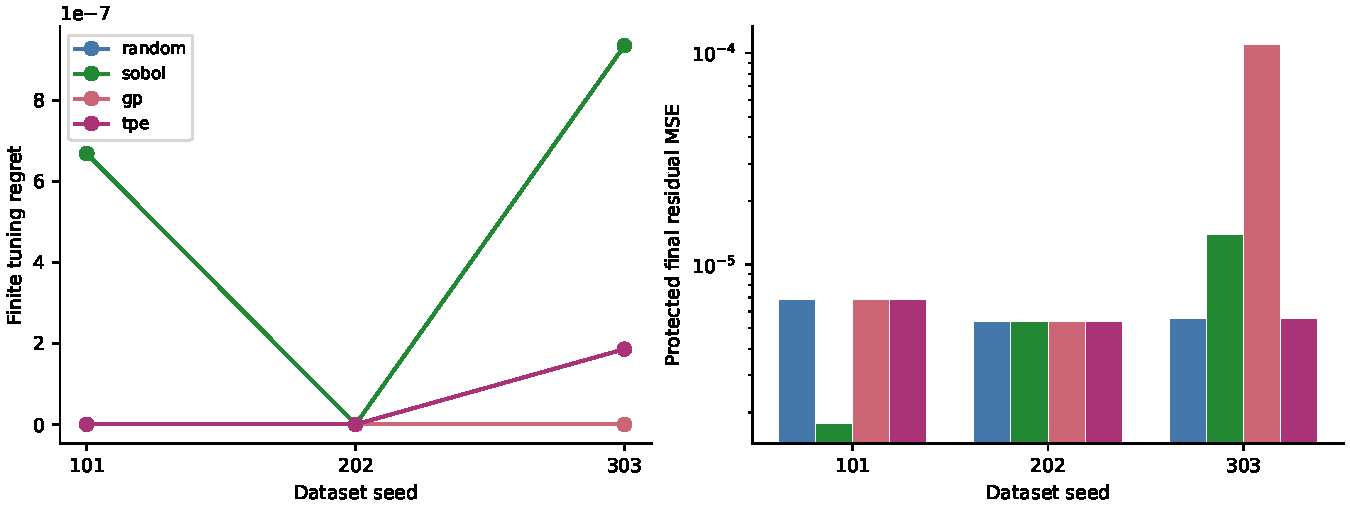
\includegraphics[width=\textwidth]{figures/doc01-results.pdf}
\caption{Observed finite tuning regret and protected final residual MSE.
Each point/bar comes from retained results. The final panel exposes sensitivity
to fresh training seeds, including the poor final fit of the tuning-optimal
small network on dataset 303. No uncertainty interval or superiority claim
is inferred from three replicates.}
\end{figure}

\section{Independent checks, recovery and reproducibility}

Independent reconstruction verified \textbf{822 fitted model artifacts}:
402 response fits and 420 neural fits, including all exhaustive-reference and
search/final fits. The checker imports neither the fitter nor PyTorch. It uses
scalar stable logistic likelihood/KKT calculations and a separate NumPy forward
pass/chain rule for neural values and derivatives, checked against central
differences. It reconstructs all finite means, selected configurations, regret,
final means, counts and charged work. All 24 studies passed completed resume
using fresh objects without new objective calls or changed report values.

Six focused test groups cover convex fitting, trained architecture changes,
analytic equilibrium substitution, disjoint roles, artifact/parameter tampering,
invalid configurations and numerical/work reconstruction. Existing qualification
separately covers interrupted core recovery; completed resume in these new
examples is not a new machine-crash experiment. Numerical conformance passing
does not turn a poor learned approximation into a good scientific result.

The source, frozen design and tests are in \path{hpo-survey/examples/}.
On the configured workspace, the exact reviewed operations are listed in
\path{docs/PROGRAM_OPERATIONS.md}. They include \texttt{doc\_ops.py test},
\texttt{response}, \texttt{equilibrium}, \texttt{verify}, \texttt{smoke} and
\texttt{build}. Use the full absolute command as written in that runbook.
The fixed runner refuses to repeat a passing allocation automatically.
For a new independent checkout with the package and TPE extra installed,
these companion commands create fresh output directories:

\begin{verbatim}
python hpo-survey/examples/application_examples.py \
  response /tmp/response-example-new
python hpo-survey/examples/application_examples.py \
  equilibrium /tmp/equilibrium-example-new
python hpo-survey/examples/independent_checks.py \
  /tmp/response-example-new
\end{verbatim}

The direct companion commands are portable examples; the reviewed workspace
runner additionally owns CPU/thread environment, outer deadlines and receipts.
The unchanged runtime was read back after execution: Python 3.13.13,
NumPy 2.5.2, SciPy 1.18.1, PyTorch 2.13.0, BoTorch 0.18.1,
GPyTorch 1.15.2 and Optuna 4.9.0. The readback records package origins,
CPU affinity and numerical thread settings; no installation or runtime change
occurred during this extension. The new quick-start smoke checks use this
checkout; the separate retained offline-wheel evidence supplies installed
Python 3.12/3.13 verification. These are distinct evidence scopes.
Companion code is distributed with the repository/manual, not the installed
wheel. Raw JSON data, models, full-grid tables, SQLite snapshots, reports,
summaries, warnings and timing logs are retained beneath
\path{docs/program/evidence/2026-10-24/doc-01/}. Provenance is listed in
\path{hpo-survey/examples/RESULTS.md}. None of the sibling applications or
private bank data is required to reproduce the mathematical examples.
